\documentclass{article}
\usepackage{tikz}

\begin{document}

To draw a ray diagram for an object placed outside the center of curvature of a concave mirror, follow these steps:

\begin{enumerate}
  \item Draw the principal axis (a horizontal line through the center of the mirror).
  \item Draw the mirror itself as a concave shape.
  \item Mark the center of curvature ($C$) on the principal axis.
  \item Place the object (an arrow, for example) outside the center of curvature on the principal axis.
  \item Draw three rays:
    \begin{enumerate}
      \item A ray parallel to the principal axis that passes through the focal point ($F$) after reflection.
      \item A ray that passes through the center of curvature ($C$) and reflects back along the same path.
      \item A ray that passes through the focal point ($F$) before reflection and becomes parallel to the principal axis after reflection.
    \end{enumerate}
  \item Where these three rays intersect after reflection, that's the position of the image. Draw the image (inverted or upright) formed.
\end{enumerate}

Characteristics of the image:

The image formed by an object placed outside the center of curvature of a concave mirror is real, inverted, and diminished in size.

\begin{center}
\begin{tikzpicture}
  % Mirror
  \draw (-4,0) arc (180:0:4);
  
  % Principal Axis
  \draw[dashed] (-6,0) -- (6,0);
  
  % Center of Curvature
  \node at (0,-0.5) {$C$};
  
  % Object
  \node at (-2,2) {Object};
  
  % Object Arrow
  \draw[->, thick] (-2,1.5) -- (-2,0);
  
  % Focal Point
  \node at (-2.5,-1) {$F$};
  
  % Rays
  \draw[dashed] (-2,0) -- (4,1);
  \draw[dashed] (-2,0) -- (-4,2);
  \draw[dashed] (-2,0) -- (-4,-2);
  
  % Image
  \node at (4,1.5) {Image};
\end{tikzpicture}
\end{center}
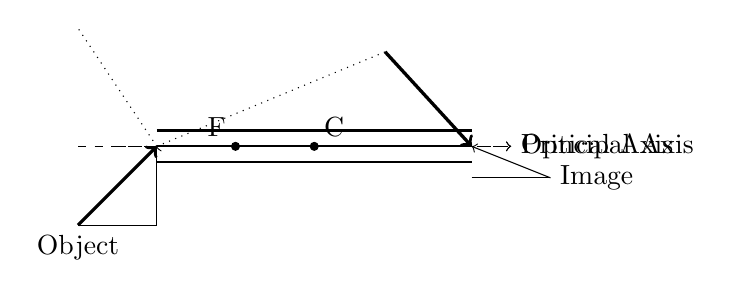
\begin{tikzpicture}
    % Drawing the mirror
    \draw[thick] (-2,0) -- (2,0);
    \draw[thick] (-2,-0.2) -- (2,-0.2);
    \draw[thick] (-2,0.2) -- (2,0.2);
    
    % Drawing the principal axis
    \draw[->, dashed] (-2.5,0) -- (2.5,0) node[right] {Principal Axis};
    
    % Drawing the center of curvature and focal point
    \draw[fill] (0,0) circle (0.05) node[above right] {C};
    \draw[fill] (-1,0) circle (0.05) node[above left] {F};
    
    % Drawing the incident ray
    \draw[->, very thick] (-3,-1) -- (-2,0);
    \draw[dotted] (-2,0) -- (0.9,1.2);
    
    % Drawing the reflected ray
    \draw[->, very thick] (0.9,1.2) -- (2,0);
    \draw[dotted] (-2,0) -- (-3,1.5);
    
    % Drawing the optical axis
    \draw[->, dashed] (-3,0) -- (2.5,0) node[right] {Optical Axis};
    
    % Drawing the object
    \draw (-3,-1) node[below] {Object} -- (-2,-1);
    \draw[->] (-2,-1) -- (-2,0);
    
    % Drawing the image
    \draw (2,-0.4) -- (3,-0.4) node[right] {Image};
    \draw[->] (3,-0.4) -- (2,0);
    
\end{tikzpicture}
\end{document}